\documentclass[a4paper,11pt]{article}
\usepackage[utf8]{inputenc}
\usepackage{textcomp}
\usepackage{lmodern}
\usepackage{listings}
\usepackage{graphicx}
\usepackage{listings}
\usepackage{color}
\definecolor{lightgray}{rgb}{0.9,0.9,0.9}
\definecolor{darkgray}{rgb}{0.4,0.4,0.4}
\definecolor{purple}{rgb}{0.65, 0.12, 0.82}
\usepackage{url}
\usepackage[top=3cm,bottom=3cm,left=3cm,right=3cm]{geometry}

\title{Royal Military Academy\\
	INFO-Y113 --- Management of Security: \\
	Concept Of Operations v2}

\author{DANHIER Piere, LECOCQ Alexis, NYAKI Loïc}

\begin{document}
\maketitle
\newpage
\tableofcontents

\newpage

\section{Introduction}
In recent years, cyber-security has become a primary concern for companies all over the world. No matter the size of the company, data often represent the heart of their business and whether the concern is the secrecy of intellectual property, or users' privacy, the theft of private data bears a huge cost for companies. Be it a monetary cost (lawsuits, fines) or a reputation cost (loss of trust, public outrage). In the case of government agencies, states secrets and other classified information could be stolen by a foreign nation, possibly leading to the loss of lives in conflict zones, loss of political leverage on the international scene, domestic political turmoil and scandals or simply public embarrassment.\\

When trying to protect these sensitive data, a common measure is be to physically isolate the network from the internet, by creating an \textit{air gap}. Acting this way ensures that the data from the network is inaccessible from the outside world. The main issue with this method is that inevitably, some external data or files will at some point need to be imported into the secure network, be it for software update, or simply because some files from the outside are necessary for the people working in the secure network. In that case, a manual import (via USB drive, by connecting an external laptop into the secure network, or by using some other data transfer device) will be necessary.\\

The problem with that method is that it can compromise the security of the secure network. For instance, the data that is manually transferred into the network may have been infected by a malware, or the secure network might already be infected by a virus. In both cases, there is a possibility for some malicious code to exfiltrate data, or to spread a virus outside, by secretly writing on the device that was originally used to import the data into the network.\\

As a consequence, we need to build a solution that prevents data leaks while allowing the transfer of files from the outside network into the secure network.

\section{Goals of the project}
\label{sec:goals}
Goals define the general direction of what the organization aims to accomplish, in the long term. Here, we wish to design a system that accomplishes two main goals :

\begin{enumerate}
\item{Create a device that completely prevents the exfiltration of data from a secure network, while allowing data to be transferred from the outside world into that secure network.}
\item{Ensure the availability of the system. The services should always be up, with no downtime}
\item{Allow specific users to manage and operate this system through an administration web page, accessible from within the secure network.}
\end{enumerate}

For this project, the general solution is imposed and should be a data diode, which we will describe in section~\ref{sec:data-diode}.


\section{Objectives}
\label{sec:objectives}
Objectives can be considered as the building parts goals. They are concrete and can be achieved by following a certain number of steps. Achieving all the objectives should translate to achieving all the goals.\\


We identify the following objectives:
\begin{itemize}
\item{Build a web interface for administrating the data diode}
\item{Use the File Transfer Protocol to implement a file transfer functionality between the outside network and the secure network.}
\end{itemize}

\subsection{Data Confidentiality}
There should be no way for data to leak outside of the secure network. Preventing physical access to a computer in the secure network is out of the scope of this project (see section \ref{sec:outscope}).\\

The objectives for ensuring data confidentiality are as follows:

\begin{itemize}
\item{Physically prevent data from exiting the secure network}
\item{When establishing communication with our system, user credentials and information shouldn't be exposed to other users.}
\end{itemize}

\subsection{Data Integrity}
The data retrieved from the outside of the network should be the same as the data that was initially sent. No data corruption or modification should take place.

\subsection{System Availability}
The system should be always up, unless it is turned off on purpose by a legitimate user or administrator.

The objectives for ensuring system availability are as follows:

\begin{itemize}
\item{The system must keep working no matter how many files are pushed to the system}
\item{An authorized user should always be able to transfer a file into the secure network}
\item{An authorized user should always be able to access and operate the administration page}
\item{In case of system crash, the system must restarted immediately}
\item{The web interface should always be accessible and working as intended. Therefore, measures should be taken against Cross site scripting (XSS) and Cross Site Request Forgery attacks (CSRF).}

\end{itemize}


\section{Scope}
It is important to precisely identify the scope of this project, in relation to our goals and objectives.\\

Our solution is destined to be integrated in an existing system. As such, when considering the security of the system as a whole, we must identify which security aspects fall under our responsibility and which don't. 

\subsection{In scope}
The following elements are in scope, which means that it is our responsibility to make sure that the security of these elements is ensured.

\begin{itemize}
\item{The availability of the file transfer service}
\item{The confidentiality of user data and credentials when interacting with the data diode (see section \ref{sec:data-diode})}
\item{The confidentiality of the data within the secure network. There should be no data leak.}
\end{itemize}

\subsection{Out of scope}
\label{sec:outscope}
The following elements are out of scope. This means that the security of these elements does not fall under our responsibility, but rather under the responsibility of the client, or another third party.

\begin{itemize}
\item{The physical access to the hardware, such as the power button or Ethernet cables}
\item{The physical integrity of the hardware}
\item{The electrical power source}
\item{The security within the secure network, such as the presence of malwares or other viruses}
\end{itemize}


\section{Data Diode}
\label{sec:data-diode}
Based on the goals and objectives specified respectively in section \ref{sec:goals} and section \ref{sec:objectives} and on the project requirements, we are going to implement a \textit{data diode}.\\

Just like a diode only conduct current in one direction, a data diode is a networking device that only allows data to flow in one direction. It is composed of two physical servers: one server communicates with the outside network and the other one communicate with the secure network. The two servers are connected together by a single unidirectional fiber optics cable.\\

A fiber optic connection normally uses two cables: one for each direction. In the case of 	 data diode, only one cable is used, allowing the data to flow in one direction. The cable going in the other direction is physically cut. As a consequence, data going through a data diode can only flow in one direction, which is required by the goals defined in section \ref{sec:goals}.

\begin{figure}
	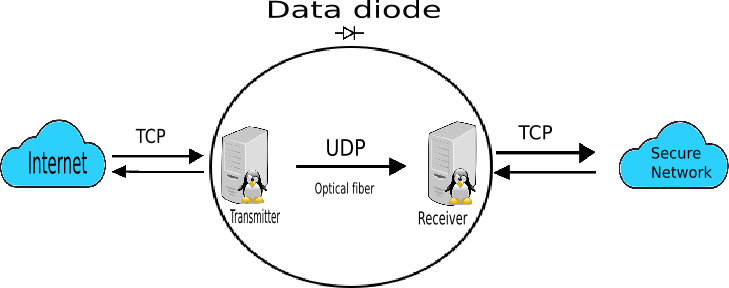
\includegraphics[scale=0.7]{img/network.png}
	\caption{High level architecture of a data diode.}
\end{figure}

\subsection{Simulating a data diode}
At first, instead of using a real data diode, we are going to build the prototype of a data diode by simulating the actual system through software. The unidirectional nature of the data transfer will be simulated by modifying the IP table in a way that will allow traffic in one direction, and drop all traffic going in the other direction.

\subsection{Applications}
With this data diode, we decided to keep things simple and to focus on proposing the two following services: a File Transfer service, as well as a data-diode administration service, as specified in our goals and objectives (section \ref{sec:goals} and section \ref{sec:objectives}).\\

Other applications such as email management and web browsing will be considered for future versions of the data-diode.

\subsubsection{File Transfer (FTP)}
The main application of this project is a file transfer service that will enable files to be pushed from the outside network into a directory situated in the inner part of the data diode, through the use of the File Transfer Protocol (FTP).\\

The management of the FTP accounts is handled by administrators through the data diode administration page, as described in section \ref{sec:administration}.

\subsubsection{Administration and User Management}
\label{sec:administration}
One of the goals of this project is the creation of a web interface for managing the data diode. We will implement an HTTP server, on the internal side of the data diode. This administration interface will allow administrators to monitor file transfers, create or delete FTP accounts as well start, stop or restart the data diode.

\subsection{Physical Architecture}
The data diode is composed of two separate servers connected to each other through a unidirectional fiber optics cable. Each server has the following components :
\begin{itemize}
\item{Two network interfaces: one for connecting to a network, and one for connecting to the other server}
\item{A fiber optic adapter, to translate the signal coming from the fiber optic cable from light into a signal that can be transmitted through an Ethernet port.}
\end{itemize}

\subsection{Software architecture}
TODO
\begin{itemize}
\item{1 FTP servers (sender). The sender must be able to receive PUT requests from the outside.}
\item{An UDP client (on the \textit{sender} side) that will send files over UDP}
\item{An UDP server (on the \textit{receiver }side)} that will receive the files pushed over TCP
\end{itemize}
\subsubsection{Technical Aspects}
A data diode is composed of two servers linked by a one-way communication channel. The server, that we'll call the \textit{sender}, receives data from the external network with the TCP protocol. The second server, called the \textit{receiver}, uses the TCP protocol to send data to the secure network too. The same conclusion can then be applied to those data.\\

The one-way communication channel between the two sides of the data-diode forbids the use of a TCP based protocol (such as HTTP or FTP), as TCP requires bi-directional communication between two parties. As data between the two sides of the data-diode can only flow in one direction, we need data to be send over a protocol that doesn't require bi-directional communication. This can be done by using UDP for the communication between our two servers. The problem with UDP is that the sender cannot be sure that the receiver received the data or if the data is not corrupted. To mitigate this risk, we chose to send three times the packets of data.


\section{Users}
We identify three types of users : the administrators, the simple users and the FTP users.
\subsection{Simple Users}
Simple users are users from inside the secure network. Their main interaction with the system is that they will need to retrieve the files that were pushed into the data diode.

\subsection{Administrators}
Administrators can monitor the system, create accounts for simple users as well as for FTP users.

\subsection{FTP Users}
FTP users operate from outside the secure network and are allowed to push files into the secure network. Each FTP user will have an account on the data diode, created by an administrator. This account allows him to push data through the data diode, via an FTP connection.

\section{Administration and Management}
\subsection{Users Administration}
\subsubsection{Simple Users}
If a user forgets his password, he has to contact the system administrator to obtain a new one.
\subsubsection{Administrators}
An administrator is able to turn on or off the data diode through the web administration page within the secure network. He also is the users and providers manager. He can create or delete a user or provider account and modify the priviliges of the accounts. 
\subsection{Data Diode Installation, Configuration and Administration}
\subsubsection{Installation}
\subsubsection{Configuration}
\subsubsection{Administration}

\end{document}